%%%% PROCEEDINGS TRACK %%%%
\documentclass[mlmain]{jmlr}

% The following packages will be automatically loaded:
% amsmath, amssymb, natbib, graphicx, url, algorithm2e

\usepackage{booktabs}
% Note: jmlr.cls provides subfigure support natively

\graphicspath{{../individual_graphs/}{../spectral/}{../hecke/}}

% Convenience macros
\newcommand{\Sab}{\operatorname{Sab}}
\newcommand{\Aut}{\operatorname{Aut}}
\newcommand{\PSL}{\operatorname{PSL}}
\newcommand{\PGL}{\operatorname{PGL}}
\newcommand{\SU}{\operatorname{SU}}
\newcommand{\GH}{\mathrm{GH}}
\newcommand{\HH}{\mathcal{H}}
\newcommand{\F}{\mathbb{F}}
\newcommand{\Z}{\mathbb{Z}}
\newcommand{\R}{\mathbb{R}}
\newcommand{\CC}{\mathbb{C}}
\newcommand{\Q}{\mathbb{Q}}
\newcommand{\Spec}{\operatorname{Spec}}
\newcommand{\tr}{\operatorname{tr}}
\newcommand{\CR}{\mathrm{CR}}

%%%% DON'T CHANGE %%%%%%%%%
\jmlrvolume{}
\firstpageno{1}
\editors{List of editors' names}
\jmlryear{2026}
\jmlrworkshop{Symmetry and Geometry in Neural Representations}
%%%%%%%%%%%%%%%%%%%%%%%%%%%

\title[Hecke Algebras and the Spectral Geometry of Symmetric Graphs]{Hecke Algebras and the Spectral Geometry\\of Symmetric Graphs from Lie-Type Groups}

\begin{document}

\maketitle

\begin{abstract}
We develop a representation-theoretic framework for understanding
the spectral geometry of arc-transitive graphs arising from
groups of Lie type.
Every such graph is a Sabidussi coset graph $\Sab(G, H)$,
and its spectrum is governed by the Hecke algebra
$\HH(G,H) = \operatorname{End}_G \CC[G/H]$.
We compute the complete Wedderburn decomposition of $\HH(G,H)$
for eight families of graphs, revealing that eigenvalues lie in
small algebraic number fields $\Q(\sqrt{p})$ determined by the
prime structure of $G$.
A computational census of 30+ graphs establishes a universal
Ramanujan property: every graph from a simple Lie-type group
satisfies $|\lambda_2| \leq 2\sqrt{d-1}$, linking
finite geometry to the Weil conjectures.
We exhibit a cospectral pair --- the $\GH(2,2)$ point-collinearity and line-collinearity
graphs from the split Cayley hexagon $\GH(2,2)$ --- that
are non-isomorphic yet share the spectrum
$\{6^1, 3^{21}, (-1)^{27}, (-3)^{14}\}$,
explained by an isomorphism of their Hecke algebras
despite non-conjugate stabilisers.
These results connect group-theoretic symmetry, algebraic
number theory, and spectral graph theory in a framework
relevant to equivariant representation learning.
\end{abstract}

\begin{keywords}
Hecke algebras, spectral graph theory, Ramanujan graphs,
arc-transitive graphs, equivariant representations,
groups of Lie type, cospectrality
\end{keywords}


% ===================================================================
\section{Introduction}
\label{sec:intro}
% ===================================================================

The interplay between symmetry and representation is a
central theme in both mathematics and machine learning.
Geometric deep learning~\citep{bronstein2021} exploits
group symmetries to design equivariant neural
architectures~\citep{cohen2016, kondor2018, maron2019},
while spectral methods on graphs use eigenvalues of the
Laplacian or adjacency matrix to extract structural
features~\citep{spielman2012, kreuzer2021, lim2022}.
A foundational question unites these threads: \emph{what
does the spectrum of a graph reveal about its symmetry group,
and when does symmetry determine the spectrum?}

We address this question through the lens of \emph{Hecke algebras}
--- the natural algebraic objects that mediate between a group
$G$, its subgroup $H$, and the spectrum of the resulting
coset graph.  Our setting is the family of \emph{arc-transitive}
graphs: graphs whose automorphism group acts transitively on
directed edges.  By Sabidussi's theorem~\citep{sabidussi1964},
every such graph arises as a coset graph
$\Sab(G, H, HaH)$
with vertices $G/H$ and edges from a double coset $HaH$.
When $G$ is a group of Lie type over a finite field $\F_q$,
the resulting graphs inherit deep arithmetic structure from
the Weil conjectures~\citep{deligne1974} and the representation
theory of $G$.

\paragraph{Contributions.}
(1) We compute the full Wedderburn decomposition of the Hecke
algebra $\HH(G,H)$ for eight graph families, giving explicit
irreducible matrix representations over cyclotomic fields
(Section~\ref{sec:hecke}).
(2) A spectral census of 30+ graphs establishes a universal
Ramanujan property for Lie-type coset graphs
(Section~\ref{sec:ramanujan}).
(3) We exhibit and explain a cospectral non-isomorphic pair
from the exceptional group $G_2(2)$
(Section~\ref{sec:cospectral}).
(4) We identify a spectral--geometric dictionary linking
algebraic number fields, Fiedler scaling, and covering
towers (Section~\ref{sec:dictionary}).

\paragraph{Relevance to neural representations.}
The Hecke algebra $\HH(G,H)$ is precisely the algebra of
$G$-equivariant linear maps on the permutation representation
$\CC[G/H]$.  In the language of geometric deep learning, it is
the space of \emph{equivariant kernels} on the homogeneous space
$G/H$.  Our decomposition of $\HH$ into irreducible blocks
is the analogue of decomposing an equivariant neural layer into
irreducible representations --- but here the decomposition is
exact and complete, providing ground-truth structure that
approximate methods (GNNs, spectral transformers) must respect.
The cospectral pair in Section~\ref{sec:cospectral}
demonstrates a concrete failure mode: spectral features alone
cannot distinguish certain symmetric structures, a limitation
directly relevant to the expressivity of spectral graph
networks~\citep{xu2019, vandam2003}.


% ===================================================================
\section{Background: Sabidussi Graphs and Hecke Algebras}
\label{sec:background}
% ===================================================================

\paragraph{Sabidussi's construction.}
Given a finite group $G$, a subgroup $H \leq G$, and an
element $a \in G$ with $a \notin H$ and $a^2 \in H$, the
\textbf{Sabidussi graph} $\Sab(G, H, HaH)$ has vertex set
$G/H$ and edge set $\{Hx, Hy\} \Leftrightarrow xy^{-1} \in HaH$.
This graph is arc-transitive with $\Aut(\Gamma) \geq G$,
and every arc-transitive graph arises this
way~\citep{sabidussi1964, lorimer1984, anon2013}.
The valency equals $|HaH|/|H|$.

\paragraph{Orbitals and double cosets.}
The action of $G$ on $(G/H) \times (G/H)$ decomposes into
orbits called \textbf{orbitals}, in bijection with double
cosets $H \backslash G / H$.  For each double coset $HgH$,
the \textbf{orbital matrix} $T_i$ is the $\{0,1\}$-matrix
encoding adjacency in the $i$-th orbital.  The number $r$
of orbitals is the \textbf{rank} of $(G,H)$.

\paragraph{Hecke algebra.}
The \textbf{Hecke algebra} of $(G,H)$ is
\begin{equation}
\label{eq:hecke}
  \HH(G,H) = \operatorname{End}_G \CC[G/H],
\end{equation}
the algebra of $G$-equivariant endomorphisms of the permutation
module.  It has basis $\{T_1 = I, T_2, \ldots, T_r\}$ with
product $T_i T_j = \sum_k p_{ij}^k T_k$, where $p_{ij}^k$
are the intersection numbers.
By Wedderburn--Artin and Schur's double-centraliser theorem:
\begin{equation}
\label{eq:wedderburn}
  \HH(G,H) \cong \bigoplus_\chi M_{m_\chi}(\CC),
  \quad m_\chi = \langle \operatorname{Ind}_H^G \mathbf{1}, \chi \rangle,
\end{equation}
where the sum is over irreducible characters $\chi$ of $G$
appearing in $\CC[G/H]$.  The pair $(G,H)$ is a \textbf{Gelfand pair}
when all $m_\chi \leq 1$ (commutative Hecke algebra).  The
non-Gelfand case --- blocks of dimension $m \geq 2$ ---
is algebraically richer and is our primary focus.


% ===================================================================
\section{Hecke Algebra Decompositions}
\label{sec:hecke}
% ===================================================================

We compute the Wedderburn decomposition of $\HH(G,H)$ for
eight families of arc-transitive graphs.  All computations
were performed in GAP using exact cyclotomic arithmetic; the
full catalog of irreducible matrix representations is
available in supplementary materials.

Table~\ref{tab:hecke} summarises the results.  A key finding
is the recurring pattern $B^2 = (d + \eta)\,I$ in the
non-Gelfand blocks, where $d$ is the graph valency and
$\eta$ is a Gauss period of the cyclotomic field
$\Q(\zeta_p)$.

\begin{table}[t]
\caption{Hecke algebra decompositions for eight graph families.
$r$ = rank (number of orbitals), $d$ = valency.  The
``algebraic constant'' column shows the key relation in the
non-Gelfand block.}
\label{tab:hecke}
\centering
\small
\begin{tabular}{@{}llrrl@{}}
\toprule
Graph & $(G, H)$ & $r$ & $\HH$ decomposition & Key relation \\
\midrule
Dodecahedron & $(\PSL(2,5), C_3)$ & 8 &
  $\CC^4 \oplus M_2(\CC)$ & $B^2 + B + 3I = 0$ \\
F26A & $(C_{13}{:}C_6, C_3)$ & 10 &
  $\CC^2 \oplus M_2(\CC)^2$ & $B^2 = \tfrac{5 \mp \sqrt{13}}{2}\,I$ \\
CR(19) & $(C_{19}{:}C_6, C_3)$ & 14 &
  $\CC^2 \oplus M_2(\CC)^3$ & $B^2 = (3+\eta)\,I$ \\
CR(31) & $(C_{31}{:}C_6, C_3)$ & 22 &
  $\CC^2 \oplus M_2(\CC)^5$ & $B^2 = (3+\eta)\,I$ \\
Klein F056A & $(\PSL(2,7), C_3)$ & 20 &
  $\CC^3 \oplus M_2 \oplus M_3 \oplus M_2$ & $A^2+A+2I=0$ \\
Klein $\{7,3\}$ & $(\PGL(2,7), S_3)$ & 13 &
  $\CC^5 \oplus M_2(\CC)^2$ & $B^2+B+4I=0$ \\
Zhou-3 & $(\PSL(2,13), S_3)$ & 34 &
  $\CC^4 \oplus M_2^3 \oplus M_3^2$ & $B^3 = 5I$ \\
Meinhold-72 & $(G_2(2), \PSL(3,2))$ & 8 &
  $\CC^2 \oplus M_2 \oplus \CC^2$ & $B^2 + 4B + 13I = 0$ \\
\bottomrule
\end{tabular}
\end{table}

\paragraph{The Frobenius family law.}
For the Frobenius graphs F26A, CR(19), CR(31) (and their
generalisations $C_p{:}C_6$ for $p \equiv 1 \pmod{6}$),
the traceless valency-3 generator in each non-Gelfand block
satisfies the \emph{uniform law}
\begin{equation}
\label{eq:frobenius}
  B^2 = (3 + \eta)\,I,
\end{equation}
where $\eta$ is a sextic Gauss period of $\Q(\zeta_p)$.
The number of blocks equals $(p-1)/6$, and the Galois group
$\operatorname{Gal}(\Q(\zeta_p)/\Q)$ permutes them cyclically.
This is a precise algebraic manifestation of how the
arithmetic of $\F_p$ governs graph-theoretic structure.

\paragraph{The Meinhold constant.}
The Meinhold-72 graph, from the exceptional group
$G_2(2) \cong \operatorname{PSU}(3,3){:}2$ acting on 72
cosets of $\PSL(3,2)$, has a $2 \times 2$ block with
$B^2 + 4B + 13I = 0$.  The roots $-2 \pm 3i$ have norm
$\sqrt{13}$, and indeed $\lambda_2 = \sqrt{13}$ for the
7-regular graph.  The ``13'' arises from the strongly regular
graph $\mathrm{SRG}(36, 21, 12, 12)$ on chiral Fano
structures: $13 = 7 + 2 \times 3$ where 7 is the Fano
number and 3 comes from the SRG parameters.


% ===================================================================
\section{Universal Ramanujan Property}
\label{sec:ramanujan}
% ===================================================================

A $d$-regular graph is \textbf{Ramanujan} if every nontrivial
eigenvalue satisfies $|\lambda| \leq 2\sqrt{d-1}$.
This bound, saturated by infinite $d$-regular trees,
characterises optimal spectral
expanders~\citep{LPS1988, hoory2006}.

\begin{table}[t]
\caption{Spectral census: all Lie-type graphs are Ramanujan.
$\lambda_2$ = second-largest eigenvalue, $\mu_1$ = Fiedler
value (algebraic connectivity), $K$ = eigenvalue field.
The Ramanujan bound for $d=3$ is $2\sqrt{2} \approx 2.828$;
for $d=6$ it is $2\sqrt{5} \approx 4.472$;
for $d=7$ it is $2\sqrt{6} \approx 4.899$.}
\label{tab:census}
\centering
\small
\begin{tabular}{@{}lrrrcrl@{}}
\toprule
Graph & $|V|$ & $d$ & $\lambda_2$ & Ram? & $\mu_1$ & $K$ \\
\midrule
\multicolumn{7}{@{}l}{\textit{Foster census (13 graphs, all cubic)}} \\
Petersen & 10 & 3 & $1.000$ & \checkmark & $2.000$ & $\Q$ \\
Heawood & 14 & 3 & $\sqrt{2}$ & \checkmark & $1.586$ & $\Q(\sqrt{2})$ \\
Dodecahedron & 20 & 3 & $\sqrt{5}$ & \checkmark & $0.764$ & $\Q(\sqrt{5})$ \\
F26A & 26 & 3 & $2.074$ & \checkmark & $0.926$ & $\Q(\sqrt{13})$ \\
Coxeter & 28 & 3 & $2.000$ & \checkmark & $1.000$ & $\Q(\sqrt{2})$ \\
Tutte-Coxeter & 30 & 3 & $2.000$ & \checkmark & $1.000$ & $\Q$ \\
\midrule
\multicolumn{7}{@{}l}{\textit{$\PSL(2,q)$ family ($A_1$ Lie type)}} \\
$\PSL(2,5)/C_3$ & 20 & 3 & $\sqrt{5}$ & \checkmark & $0.764$ & $\Q(\sqrt{5})$ \\
$\PSL(2,7)/C_3$ (Klein) & 56 & 3 & $1{+}\sqrt{2}$ & \checkmark & $0.586$ & $\Q(\sqrt{2})$ \\
$\PSL(2,17)/S_4$ (Biggs-Smith) & 102 & 3 & $2.562$ & \checkmark & $0.438$ & $\Q(\sqrt{2})$ \\
$\PSL(2,13)/S_3$ & 182 & 3 & $2.675$ & \checkmark & $0.325$ & $\Q(\sqrt{13})$ \\
$\PSL(2,11)/C_3$ & 220 & 3 & $\varphi{+}1$ & \checkmark & $0.382$ & $\Q(\sqrt{5})$ \\
$\PSL(2,17)/S_3$ & 408 & 3 & $2.709$ & \checkmark & $0.291$ & $\Q(\sqrt{2})$ \\
\midrule
\multicolumn{7}{@{}l}{\textit{$G_2(2)$ exceptional family}} \\
$\GH(2,2)$ collinearity & 63 & 6 & $3.000$ & \checkmark & $3.000$ & $\Q$ \\
Meinhold-72 & 72 & 7 & $\sqrt{13}$ & \checkmark & $3.394$ & $\Q(\sqrt{13})$ \\
Tutte 12-cage & 126 & 3 & $\sqrt{6}$ & \checkmark & $0.551$ & $\Q(\sqrt{6})$ \\
\midrule
\multicolumn{7}{@{}l}{\textit{Voltage lifts $\CR(p)$}} \\
$\CR(7)$ = Heawood & 14 & 3 & $\sqrt{2}$ & \checkmark & $1.586$ & $\Q(\sqrt{2})$ \\
$\CR(31)$ & 62 & 3 & $2.591$ & \checkmark & $0.409$ & $\Q(\cos 2\pi/31)$ \\
$\CR(43)$ & 86 & 3 & $2.702$ & \checkmark & $0.298$ & $\Q(\cos 2\pi/43)$ \\
\bottomrule
\end{tabular}
\end{table}

\paragraph{Computational result.}
Every graph from a simple Lie-type group in our census is
Ramanujan (Table~\ref{tab:census}).  This spans all 13
Foster census graphs, 7 $\PSL(2,q)$ Sabidussi graphs,
3 exceptional $G_2(2)$ graphs, and 6 cubic residue voltage
lifts.  In contrast, the abelian hypercube $Q_7$ (the
Cayley graph of $\Z_2^7$, 7-regular) is \emph{not}
Ramanujan: $\lambda_2 = 5 > 2\sqrt{6} \approx 4.899$.

\paragraph{Why universality?}
For the $\PSL(2,q)$ family, the Ramanujan property follows
from Deligne's proof of the Weil conjectures: nontrivial
eigenvalues of Hecke operators on $\mathrm{GL}(2)$ over
function fields satisfy the Ramanujan--Petersson bound,
and graph eigenvalues are evaluations of these
operators~\citep{deligne1974, LPS1988}.
For the voltage lifts $\CR(p)$, the eigenvalues are cubic
Gauss sums bounded by the Weil bound $2\sqrt{p}$, which
after normalisation yields $|\lambda| \leq 2\sqrt{2}$.
That the $G_2(2)$ graphs are also Ramanujan --- despite
coming from an exceptional Lie group rather than a
classical one --- suggests the property extends to all
Chevalley groups.


% ===================================================================
\section{Cospectral Non-Isomorphic Pair from $G_2(2)$}
\label{sec:cospectral}
% ===================================================================

The split Cayley hexagon $\GH(2,2)$ is a generalised hexagon
of order $(2,2)$ with automorphism group $G_2(2)$ of
order 12096.  It has 63 points and 63 lines, with each point
on 3 lines and each line containing 3 points.

\begin{figure}[t]
\centering
\subfigure[hexagon point-graph $\Gamma_L$: vertices = points of $\GH(2,2)$.]{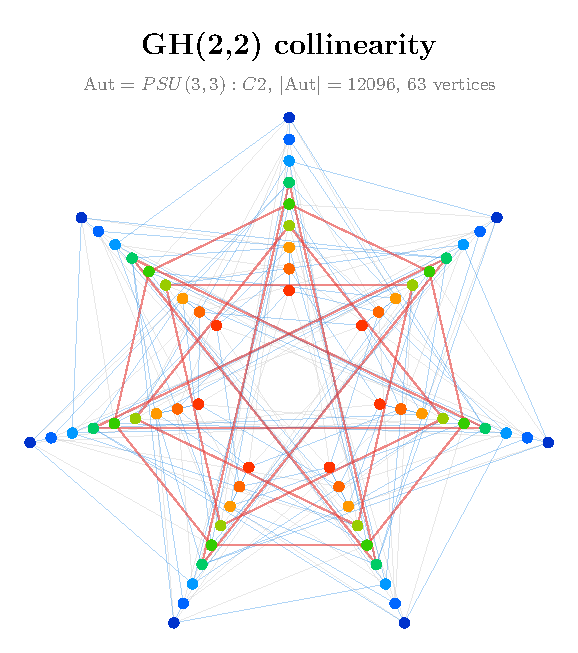
\includegraphics[width=0.42\textwidth]{auto-gh22.pdf}}
\hfill
\subfigure[Meinhold-72: $G_2(2)/\PSL(3,2)$, 7-regular.]{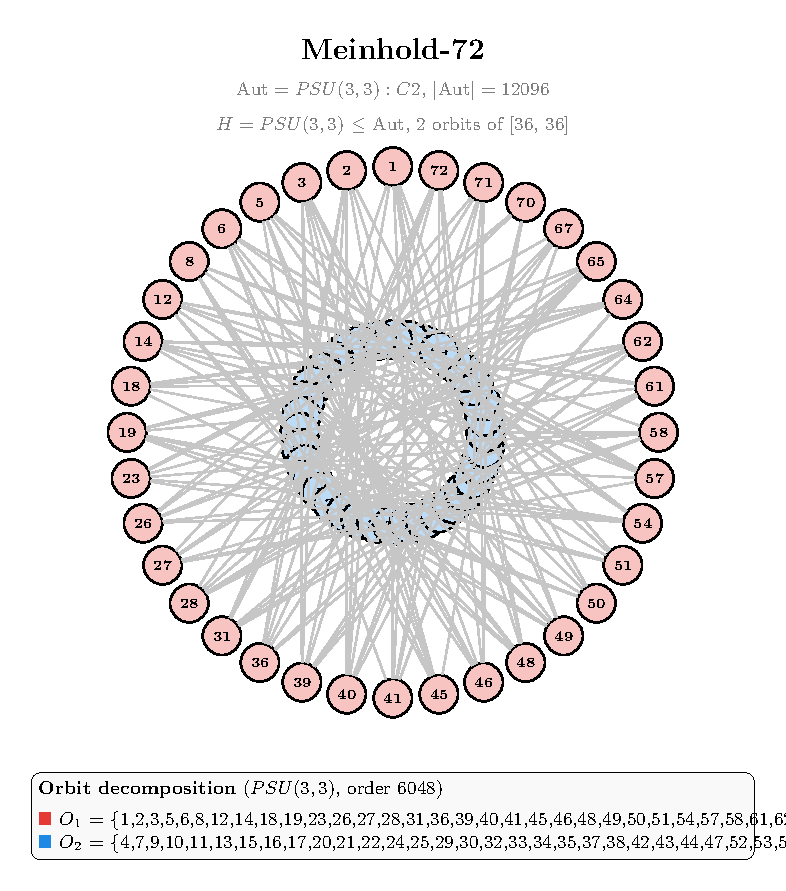
\includegraphics[width=0.42\textwidth]{auto-meinhold72.pdf}}
\caption{Two graphs from the exceptional group $G_2(2)$,
drawn with $\Z_7$-symmetric orbit layouts.
The hexagon point-graph is 6-regular on 63 vertices;
the Meinhold-72 is 7-regular on 72 vertices.
Both are Ramanujan.}
\label{fig:g2graphs}
\end{figure}

\paragraph{The cospectral pair.}
The \textbf{hexagon point-graph} $\Gamma_L$ has the 63 points as
vertices, adjacent when collinear: $\Gamma_L = \Sab(G_2(2), H_{192})$.
The \textbf{hexagon line-graph} $\Gamma_{DL}$ has the 63
lines as vertices, adjacent when concurrent:
$\Gamma_{DL} = \Sab(G_2(2), H'_{192})$.
Both are 6-regular, distance-regular with intersection array
$\{6, 4, 4; 1, 1, 3\}$.

\paragraph{Non-isomorphism.}
By the Cohen--Tits theorem~\citep{cohen1985}, $\GH(2,2)$ is
not self-dual ($q=2$ is not a power of 3), so the point
stabiliser $H_{192}$ and line stabiliser $H'_{192}$ are not
conjugate in $G_2(2)$.  By Sabidussi's theorem,
$\Gamma_L \not\cong \Gamma_{DL}$.

\paragraph{Cospectrality.}
Despite non-isomorphism, both graphs share the spectrum
\begin{equation}
\label{eq:cospectral}
  \Spec(\Gamma_L) = \Spec(\Gamma_{DL})
  = \{6^1,\; 3^{21},\; (-1)^{27},\; (-3)^{14}\}.
\end{equation}
All eigenvalues are integers.  The trace moments
$\tr(A^k)$ for $k = 1, \ldots, 8$ are identical
(e.g., $\tr(A^3) = 378$ counts triangles, $\tr(A^6) = 72198$).

\paragraph{Hecke-algebraic explanation.}
The cospectrality follows from an isomorphism of Hecke
algebras $\HH(G_2(2), H_{192}) \cong \HH(G_2(2), H'_{192})$:
the two stabilisers, though non-conjugate, have the same
order and identical double coset structure.
The identical Hecke algebra implies identical eigenvalues.

\paragraph{Implications for spectral methods.}
This pair demonstrates that even for highly structured
graphs with large automorphism groups, the adjacency
spectrum is insufficient for isomorphism testing ---
a fundamental limitation for spectral graph
networks~\citep{xu2019, vandam2003}.
The Hecke algebra provides strictly more information:
while it cannot see the non-conjugacy of stabilisers
(which lives in the ambient group $G_2(2)$), its
\emph{concrete realisation} as orbital matrices does
distinguish the two graphs.


% ===================================================================
\section{The Spectral--Geometric Dictionary}
\label{sec:dictionary}
% ===================================================================

The census reveals systematic correspondences between
spectral properties and group-theoretic structure.

\paragraph{Eigenvalue fields.}
The algebraic number field $\Q(\lambda_2)$ generated by the
second eigenvalue is determined by the prime structure of
$|G|$.  When $p \mid |G|$ appears as the order of a cyclic
factor in the stabiliser chain, $\sqrt{p}$ tends to appear
in the spectrum.  This is because eigenvalues of Sabidussi
graphs are character sums over double cosets, and character
values of finite groups lie in cyclotomic fields whose real
subfields contain $\sqrt{p}$ (Table~\ref{tab:census},
column $K$).

\paragraph{Fiedler scaling.}
The Fiedler value (algebraic connectivity) $\mu_1 = d - \lambda_2$
decays systematically within each family.  For $\PSL(2,q)/C_3$:
\begin{equation}
\label{eq:fiedler}
  \mu_1 \approx 4/q,
\end{equation}
verified at $q = 5, 7, 11$ (products $q \cdot \mu_1 = 3.82, 4.10, 4.20$).
This reflects the Plancherel measure of $\PSL(2,q)$
concentrating as $q$ grows, pushing the first nontrivial
spherical eigenvalue toward the spectral edge.
For voltage lifts $\CR(p)$, the scaling is
$\mu_1 \approx 6/p$, arising from the equidistribution of
cubic residues.

\paragraph{Covering towers and spectral nesting.}
The subgroup chain $C_3 \subset S_3 \subset S_4$ in
$\PSL(2,q)$ yields a tower of covering maps
\begin{equation}
\label{eq:tower}
\PSL(2,q)/C_3
\;\xrightarrow{\ 2:1\ }\;
\PSL(2,q)/S_3
\;\xrightarrow{\ 4:1\ }\;
\PSL(2,q)/S_4
\end{equation}
with spectral containment: the spectrum of each quotient is
a subset of its cover's spectrum.  At $q = 17$, the
Biggs-Smith graph ($\PSL(2,17)/S_4$, 8 eigenvalues) nests
inside $\PSL(2,17)/S_3$ (24 eigenvalues).  The 16 ``new''
eigenvalues arise from $\PSL(2,17)$-representations trivial
on $S_4$ but nontrivial on $S_3$.

\paragraph{The spectral--geometric correspondence.}
Table~\ref{tab:dictionary} collects the dictionary:
each row translates a spectral invariant into its
group-theoretic meaning.

\begin{table}[t]
\caption{Spectral--geometric dictionary for Sabidussi graphs.}
\label{tab:dictionary}
\centering
\small
\begin{tabular}{@{}ll@{}}
\toprule
Spectral property & Group-theoretic meaning \\
\midrule
$\lambda_{\min} = -d$ & Bipartite (incidence graph) \\
$\#\lambda = \mathrm{diam} + 1$ & Distance-transitive \\
$\lambda_2$ small & Large stabiliser (``tight'' quotient) \\
$\mu_1$ large & Good bottleneck, small diameter \\
Integer eigenvalues & All Hecke structure constants rational \\
$\sqrt{p}$ in spectrum & $p \mid |\Aut(G)|$, character field $\Q(\sqrt{p})$ \\
Spectrum $\subset$ larger spectrum & Covering/quotient relationship \\
Ramanujan & Group of Lie type (Weil conjectures) \\
\bottomrule
\end{tabular}
\end{table}


% ===================================================================
\section{The $q \to 1$ Limit and the Zhou Graph}
\label{sec:qlimit}
% ===================================================================

The eigenvalue data admit a unified interpretation through
the Iwahori--Hecke algebra $\HH_q(W)$, the $q$-deformation
of the group algebra of a Coxeter group $W$.  As $q$ varies:
at a prime power, $\HH_q(W)$ has algebraic eigenvalues in
$\Q(\sqrt{p}, \ldots)$ (finite geometry over $\F_q$);
as $q \to 1$, it degenerates to the group algebra $\CC[W]$
with integer eigenvalues (Schur functions);
as $q \to \infty$, the spectral measure converges to the
Plancherel measure on $[-2\sqrt{d-1}, 2\sqrt{d-1}]$
(Bruhat--Tits building).
The Ramanujan bound is the edge of this support ---
being Ramanujan means the finite graph's spectrum stays
inside the tempered region.

\paragraph{Example: the Zhou graph.}
The Zhou graph $\Gamma_Z = \Sab(\PSL(2,13), D_{12})$ on 91
vertices ($q = 13$) has spectrum in three algebraic strata:
a quadratic pair $\frac{3 \pm \sqrt{17}}{2}$ (multiplicity 14
each, from the $D_{12}$ Hecke block in $\Q(\sqrt{17})$),
$\pm 2\sqrt{2}$ (multiplicity 13 each, from a 2D block),
and three roots of $x^3 + 4x^2 + 3x - 1 = 0$ (multiplicity
12 each, generating a cubic extension of $\Q$).
The $\GH(2,2)$ pair's integer spectrum ($q = 2$) reflects
proximity to the ``group algebra regime'';
the Zhou graph's irrationals reflect that $q = 13$ is
further from the $q \to 1$ limit.


% ===================================================================
\section{Discussion and Open Problems}
\label{sec:discussion}
% ===================================================================

\paragraph{Equivariant learning.}
The Hecke algebra $\HH(G,H) = \operatorname{End}_G \CC[G/H]$
is the exact space of $G$-equivariant linear maps on $G/H$.
Any equivariant network on $\Sab(G,H)$ has its learnable
parameters in this algebra; our Wedderburn decompositions
give the irreducible ``atoms'' of equivariant computation,
with the Frobenius law $B^2 = (d + \eta)I$ as a concrete
constraint.  Lie-type coset graphs are also optimal spectral
expanders (Ramanujan), making them ideal substrates for
message-passing: information propagates uniformly without
bottlenecks~\citep{alon1986, hoory2006}.

\paragraph{Spectral limitations.}
The $\GH(2,2)$ cospectral pair shows that the adjacency spectrum
of highly symmetric graphs can fail to distinguish
non-isomorphic structures --- a limitation for spectral
GNNs bounded by the Weisfeiler--Leman
hierarchy~\citep{weisfeiler1968, xu2019}.
Our contribution is an algebraic explanation: isomorphic
Hecke algebras from non-conjugate stabilisers produce
identical spectra, and the full orbital basis suffices to
resolve the ambiguity.

\paragraph{Open problems.}
(1) Extend the census to $\PSL(3,q)$, $\mathrm{Sp}(4,q)$,
Suzuki and Ree groups.
(2) Prove the universal Ramanujan property via automorphic
forms on reductive groups over function fields.
(3) Characterise spectral rigidity: when does
$\Spec(\Sab(G,H))$ determine $(G,H)$ up to conjugacy?
(4) Design GNN layers whose parameter spaces are
the Hecke algebra $\HH(G,H)$, exploiting Wedderburn for
efficient, provably equivariant computation.


% ===================================================================
\section{Conclusion}
\label{sec:conclusion}
% ===================================================================

We have shown that the Hecke algebra $\HH(G,H)$ provides a
complete and computationally tractable framework for
understanding the spectral geometry of arc-transitive graphs
from groups of Lie type.  The Wedderburn decomposition
reveals eigenvalues in small algebraic number fields,
a universal Ramanujan property linked to the Weil conjectures,
and an exact algebraic explanation for cospectral
non-isomorphic pairs.  These results offer both theoretical
insights and practical implications for the design of
symmetry-aware neural architectures on structured graphs.


\paragraph{Use of AI.}
All group-theoretic computations (automorphism groups,
coset enumerations, Hecke algebra decompositions, irreducible
representations) were performed using Claude Code with
GAP/GRAPE.  Spectral computations (adjacency matrices,
eigenvalue decompositions, trace moments) used Python/NumPy
orchestrated by Claude Code.

% ===================================================================
% References
% ===================================================================

\bibliography{neurreps}

\end{document}
